% ! TeX root = ../thesis-main.tex
%----------------------------------------------------------------------------------------
\chapter{State of the art}
\label{chap:state-of-the-art}
%----------------------------------------------------------------------------------------

In the field of aggregate programming\cite{aggregate-programming}, multiple frameworks, tools, and experiments have been developed and made available as public resources to support a wide variety of use cases, using different languages and design approaches.
%
Some of the prominent examples, that can be considered state of the art, are \textit{ScaFi}\footnote{\url{https://github.com/scafi/scafi}}\cite{scafi}, \textit{Protelis}\footnote{\url{https://github.com/Protelis/Protelis}}\cite{protelis} and, \textit{FCPP}\footnote{\url{https://github.com/fcpp/fcpp}}\cite{fcpp}.
%
In this chapter, each of these tools is briefly described in their fundamental characteristics, with a particular emphasis on ScaFi, which constitutes the direct parent to \this, as discussed in \Cref{chap:background}.

Each of these libraries is backed by a solid, coherent theoretical foundation, that provides theoretical consistency and guarantees the emergence of fundamental properties in derived work.
%
This theoretical foundation that serves as the basis for all cited implementations is the \ac{FC}\cite{fc}, in particular its higher-order version, the \ac{HFC}\cite{hofc}.
%
\ac{FC}, as well as its variants, is a type-safe, formal language for aggregate programming\cite{fc, from-dc-to-fc-and-ap} presented with its operational and denotational semantics, respectively describing the local and global interpretation of field expressions\cite{from-dc-to-fc-and-ap}.
%
The key aspect of \ac{FC} is the possibility, from a developer perspective, to focus on the denotational semantics of field constructs, completely abstracting away from the local interpretation of expressions and implementation of the constructs.
%
In recent years, a new formal language has been developed, called \ac{XC}\cite{xc}, which is a promising evolution of \ac{FC} that has the potential to supersede \ac{FC} entirely given that \ac{XC} is a simpler yet more expressive language that can be used to implement all the \ac{FC} constructs while retaining their original semantics.
%
\this, as well as FCPP in its current version, is based on this newer formal language, further described in \Cref{chap:background}, where \ac{FC} and \ac{XC} are briefly compared.
%
Some additional experiments with the implementation of \ac{XC} already exist, such as \textit{imperative-xc}\footnote{\url{https://github.com/cric96/imperative-xc}} and \textit{XC: Scala DSL Implementation}\footnote{\url{https://github.com/scafi/artifact-2021-ecoop-xc}}\cite{xc-experiment-with-scafi}, described in \Cref{chap:state-of-the-art->sec:xc} and \Cref{chap:state-of-the-art->sec:imperative-xc}, respectively.

\section{Protelis}

Protelis is an external domain-specific language derived from the discontinued \textit{Proto}, whose syntax resembles that of C or Java, but it's purely functional, albeit dynamically typed and interpreted by a virtual machine written in Java\cite{protelis}.
%
As external \ac{DSL}, Protelis syntax is close to the \ac{FC} language it implements, which distinguishes it from ScaFi and FCPP, which are internal \acp{DSL}.
%
As a result, domain branching in Protelis is transparent in its conditional control syntax, such as the \texttt{if} statement, while in internal \acp{DSL} the same feature must be achieved with a custom operator to avoid conflicts with the host language's homonymous constructs.
%
More information on domain branching can be found in \Cref{chap:background->sec:xc->subsec:alignment}.
%
Nevertheless, the Protelis environment comes with some costs, such as a lack of compiler support for type checking, given that Protelis uses duck typing, and IDE support exclusively for the Eclipse platform, given that Protelis is based on the Xtext framework\cite{xtext}.
%
Additionally, external \acp{DSL} can't benefit from the community of developers and libraries of a general-purpose language such as Scala or C++, which are the host languages for ScaFi and FCPP, respectively.

An example of a gradient distance written with Protelis can be found in \Cref{lst:gradient-distance-protelis}.

\lstinputlisting[language=Protelis, caption={Gradient distance from a source in Protelis.}, label={lst:gradient-distance-protelis}]{listings/protelis-gradient-distance.pt}

\section{FCPP}

FCPP is an internal domain-specific language written in C++, originally based on \ac{FC} but already updated to support \ac{XC}\cite{xc}.
%
FCPP is oriented towards efficiency and performance, to target devices with limited resources, such as microcontrollers and embedded systems\cite{fcpp}.
%
As stated in the paper, FCPP suffers more limitations than ScaFi when it comes to avoiding conflicts with the host language, resulting in a less \quotes{clean} syntax, and it lacks integration with the Java environment, natively supported by the Scala language, which is the host language for ScaFi\cite{fcpp}.
%
Another important difference in the design of FCPP from ScaFi is the presence of explicit \texttt{field} types, which are absent in ScaFi thanks to its design around \texttt{foldhood} operations, as described in \Cref{chap:state-of-the-art->sec:scafi}.

An example of a gradient distance written with FCPP can be found in \Cref{lst:gradient-distance-fcpp}.

\lstinputlisting[language=C++, caption={Gradient distance from a source in FCPP.}, label={lst:gradient-distance-fcpp}]{listings/fcpp-gradient-distance.cpp}

\section{ScaFi} \label{chap:state-of-the-art->sec:scafi}

\textit{ScaFi} (\textit{Sca}la \textit{Fi}elds) is an aggregate programming framework featuring an internal \ac{DSL} written in pure Scala 2\cite{scafi}.
%
Besides the \ac{DSL}, which represents the core of ScaFi, the framework offers additional components for the simulation, visualization, and deployment of aggregate programs.

TODO describe ScaFi in depth

\begin{figure}
    \centering
    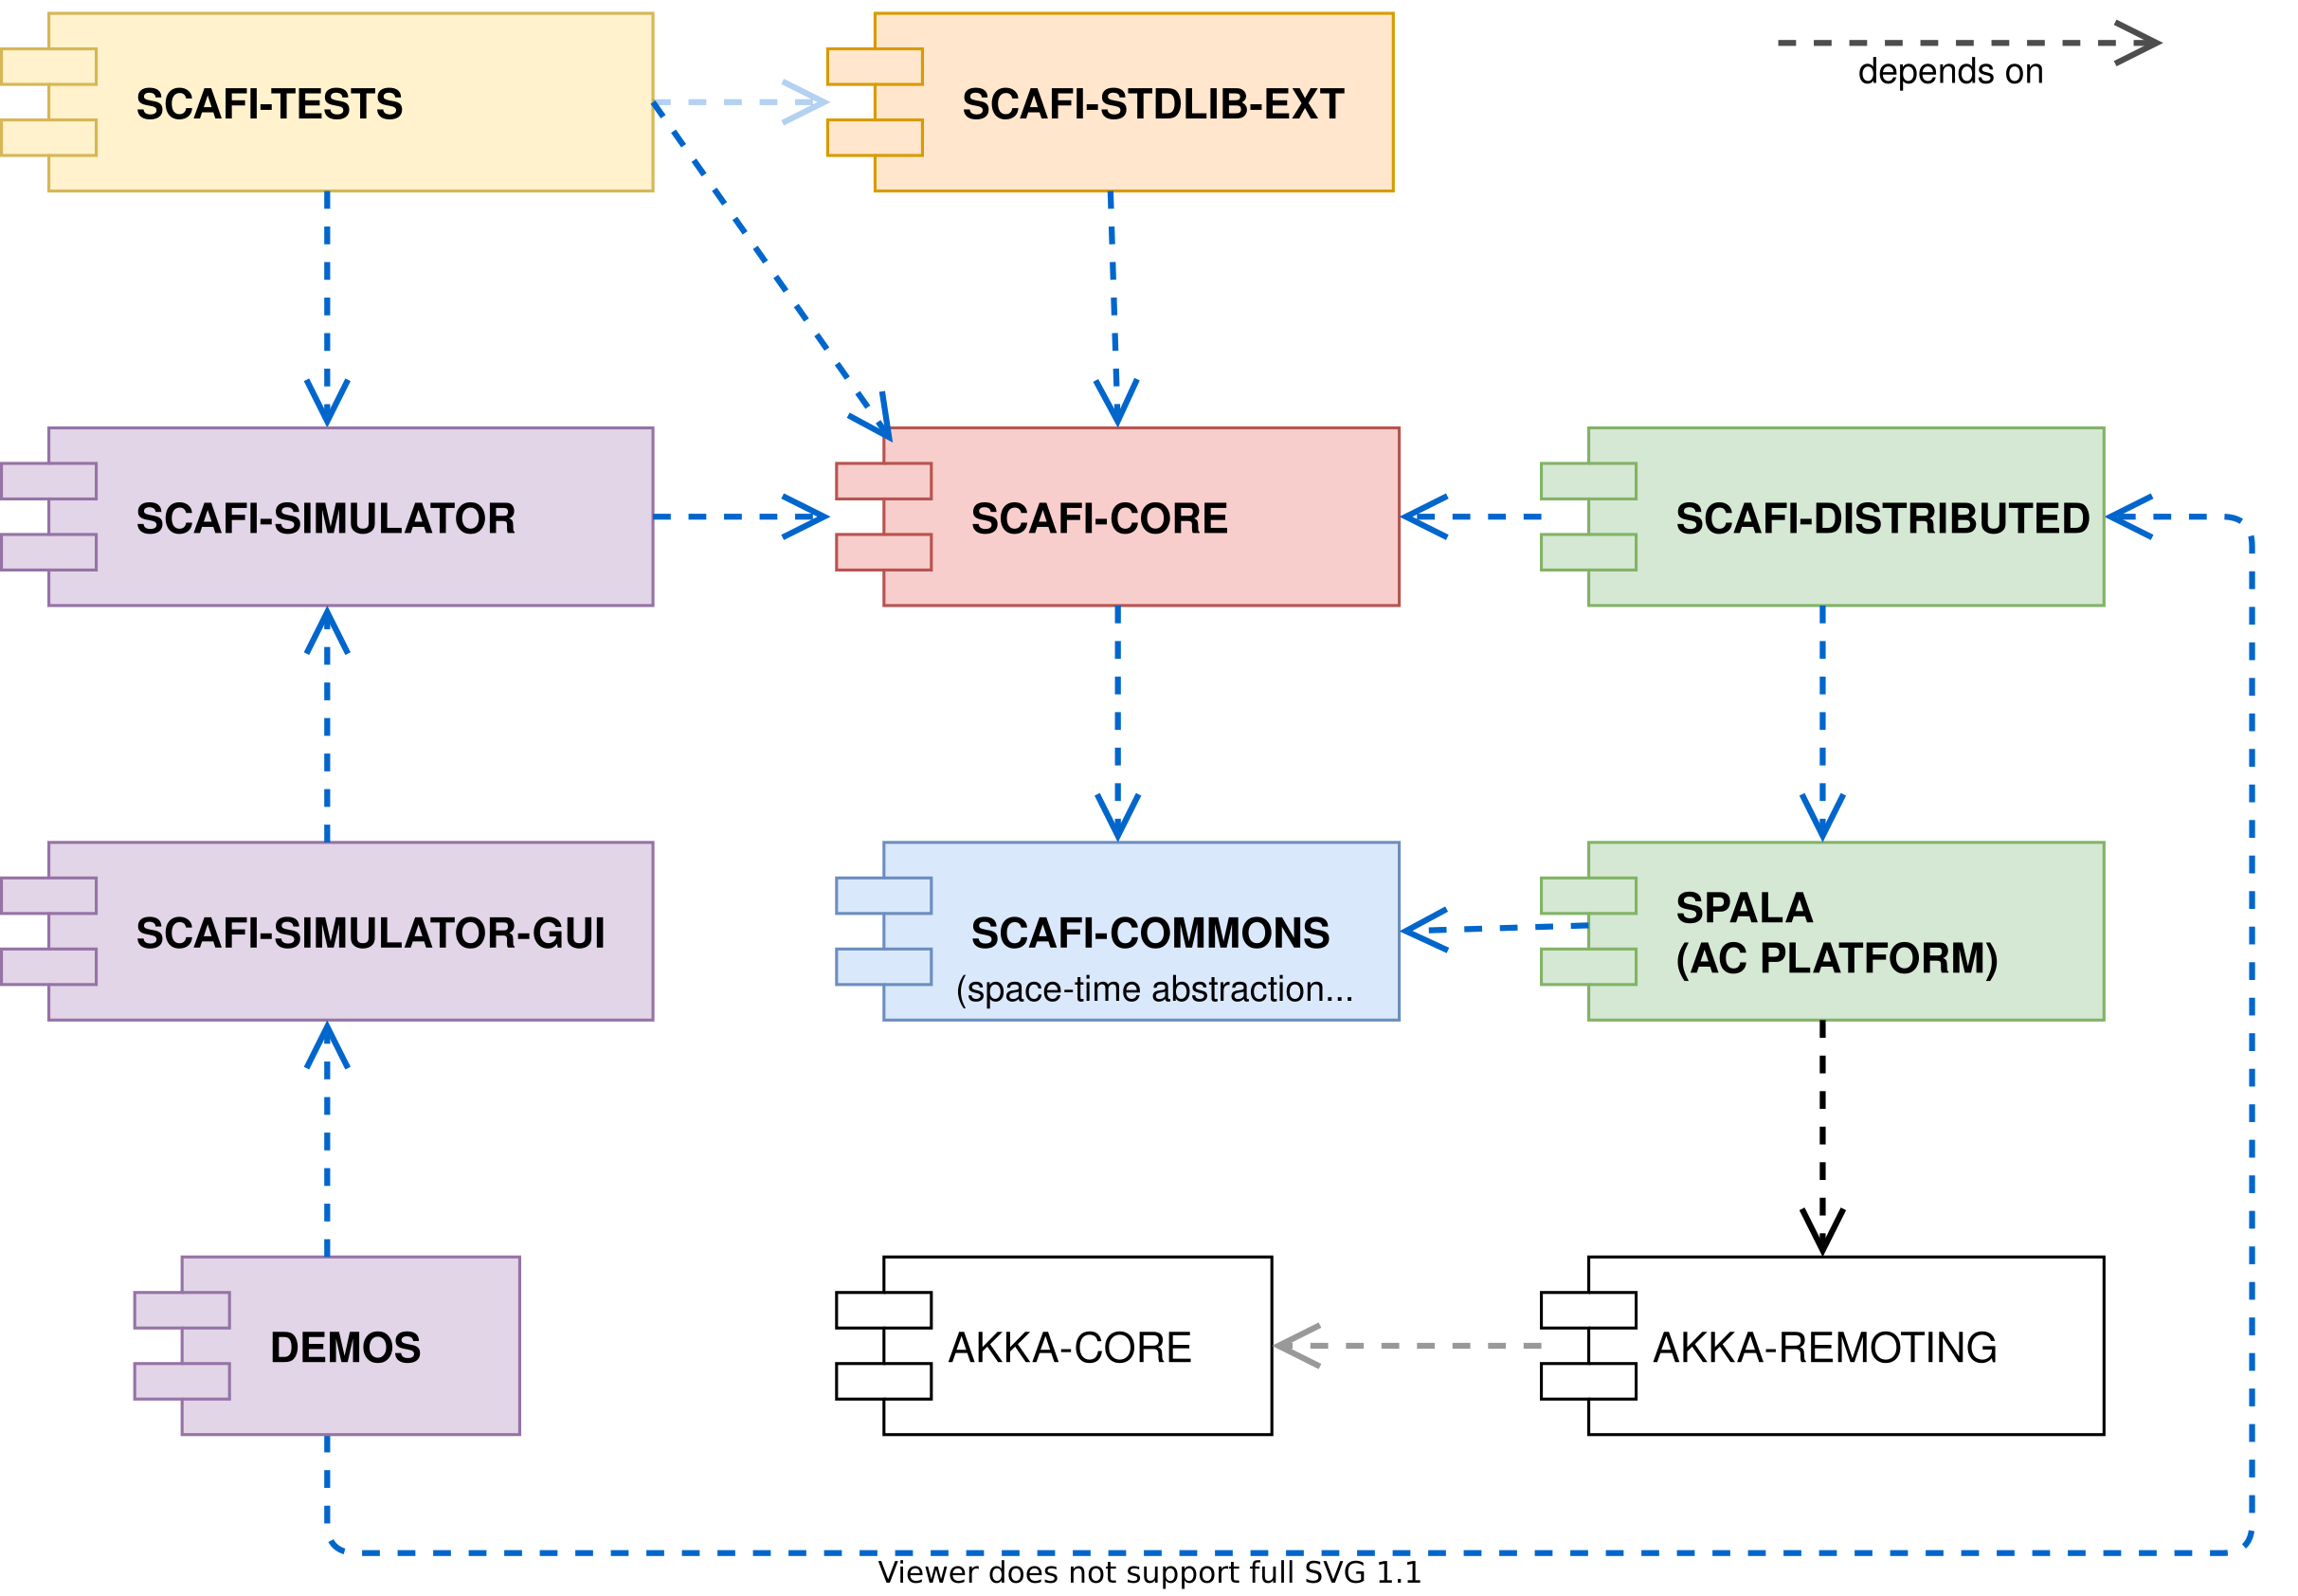
\includegraphics[width=.8\linewidth]{figures/scafi-project-org.drawio.png}
    \caption{ScaFi project organization.}
    \label{fig:random-image2}
\end{figure}

\section{XC: Scala DSL Implementation} \label{chap:state-of-the-art->sec:xc}

The first implementation of \ac{XC} in Scala is based on ScaFi and presented in the \ac{XC} papers\cite{xc}\cite{xc-experiment-with-scafi}.
%
This implementation uses Scala 2.
%
Even though ScaFi hides the \texttt{field} abstraction from the user, in this experiment \textit{NValue}s had to be explicitly implemented, given the new semantics they provide.
%
The automatic conversion from local values to nvalues, explained in the \ac{XC} paper and in \Cref{chap:background->sec:xc->subsec:nvalues}, has been implemented seamlessly thanks to Scala 2 implicit conversions.
%
In the experiment, publicly available on GitHub\footnote{\url{https://github.com/scafi/artifact-2021-ecoop-xc}} under the Apache 2.0 License and on Zenodo\cite{xc-experiment-with-scafi-code}, the \ac{FC} constructs have been implemented using \texttt{exchange}, the only communication primitive of \ac{XC}, suggesting a new syntax for a pure Scala \ac{XC}, later taken as inspiration for \this.

An example of a gradient distance written with this DSL can be found in \Cref{lst:gradient-distance-xc-scala2-dsl}.

\lstinputlisting[language=Scala, caption={Gradient distance from a source in XC Scala 2 DSL.}, label={lst:gradient-distance-xc-scala2-dsl}]{listings/xc-experiment-scafi-gradient-distance.scala}

\section{imperative-xc} \label{chap:state-of-the-art->sec:imperative-xc}
TODO write
